

\section{Gradient-based learning}
\subsection{Back-propagation}
\textbf{Denominator Layout}: $F: \mathbb{R}^d\to\mathbb{R}^m \implies \nabla_xF(x)\in\mathbb{R}^{d\times m}$\\
$\frac{\partial L}{\partial z_1}=\frac{\partial L}{\partial h_1}\text{diag}(f^\prime(z_1))=\frac{\partial L}{\partial h_1}\odot f^\prime(z_1)$, $f$ element-wise activation function\\


\textbf{Per-layer Gradients in DNN}: \(\frac{\partial x^l_ {i}}{\partial w^l_{ij}} = \frac{\partial \phi^l (W^l x^{l-1}+b^l)}{\partial w^l_{ij}} = \overset{.}{
\phi
}^l_i x^{l-1}_j \)
\(\frac{\partial x^l_i}{\partial b^l_i} = \overset{.}{\phi_i^l}\) ; Where \(\overset{.}{\phi_i^l} \equiv \) sensitivity of i-th unit in l-th layer $=\overset{.}{\phi^l}((w^l_{i})^\top x^{l-1}+b^l)$ \\
We observe that gradients only flow through \(x^{l-1}\rightarrow x^l\)  which reflects \textbf{locality} of backprop in terms of units and layers.\\
Downpropagating the changes to the loss with chain rule gives:\\ \(\frac{\partial
h[\theta](x,y)}{\partial w^l_{ij}} = \frac{\partial h^l[\theta](x^l,y)}{\partial x^l_i}\frac{\partial x^l_i}{\partial w^l_{ij}}=\delta^l_i \overset{.}{\phi_i^l}x_j^{l-1}\)
and \(\frac{\partial
h[\theta](x,y)}{\partial b^l_{i}} = \delta^l_i \overset{.}{\phi_i^l}\)\\
\textbf{note:} \(\delta^l_i \equiv \frac{\partial h^l[\theta](x^l,y)}{\partial x^l_i }\) and \(h^l[\theta](x^l,y) \equiv \ell (y, (F^L \circ \dots \circ F^{l+1})(x^l))  \)
\begin{itemize}
    \item $\delta$ describes the sensitivity of the loss to the i-th unit from the l-th layer
    \item $h^l$ is the subsequent loss after forward-prop
    \item \textbf{Linear layers} sensitivity $\overset{.}{\phi}= 1$ and  $\frac {\partial h[\theta](x^l,y)}{\partial w_{ij}^l}=\delta^l_i\times x^{l-1}_j $
    \item \textbf{Logistic layers}: $\overset{.}{\sigma}(z)=\sigma(z)(1-\sigma(z))$. Maximal sensitivity (\(\frac{1}{4}\)) at $z=0$
    \begin{itemize}
        \item Large $|z|$ cause small sensitivities, complicating optimization
    \end{itemize}
    \item \textbf{ReLU}: Deriv. is 1 f $z>0$ and 0 if $z<0$. Subderiv. $\in [0;1]$ for $z=0$
\end{itemize}
Computing \(\delta^l\) :
\begin{enumerate}
    \item $\delta^L=\frac{\partial \ell(\hat{y},y)}{\partial \hat{y}}$ e.g., for \(\ell = 1/2(y-\hat{y})^2\), \(\delta^L = \hat{y}-y\) 
    \item \(\delta^l=[\frac{\partial F^{l+1}}{\delta x^l}]^\top\delta^{l+1}\), where \(\frac{\partial F}{\partial x}= (\frac{\partial F_i}{\partial x_j })_{ij}\)
    \begin{enumerate}
        \item So, all $\delta^l$ terms can be obtained by propagating the initial loss through the transposed Jacobi matrices
        \item For $F(x) = \phi(Wx+b)$. \(\frac{\partial F}{\partial x}=  diag(\overset{.}{\phi}(Wx+b)))W\)
    \end{enumerate}

\end{enumerate}
Backpropagation can be applied to any DAG\\
\textbf{Deep Linear Networks}
\begin{itemize}
    \item $\frac{\partial\frac{1}{2}||W^L\dots W^1x-y||^2}{\partial W^l}= [W^L \dots W^{l+1}]^\top\delta x^\top [W^{l-1}\dots W^1]^\top$
    \begin{itemize}
        \item \(\delta \equiv W^L\dots W^1x-y\)
    \end{itemize}
    \item Aggregating gradients in linear (LS) networks over sets of examples yields a dependence on a set of sufficient statistics
    \begin{itemize}
        \item $\Sigma \equiv \mathbf{E}(xx^\top)$ , \(\Gamma \equiv \mathbf{E}(xy^\top)\)
        \item Where \(\mathbf{E}\) is the empirical average over a training set
    \end{itemize}
\end{itemize}
%\textbf{Examples}
%\rotatebox{90}{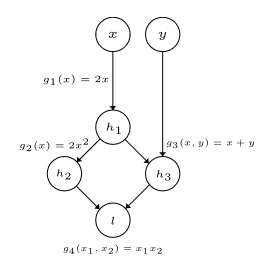
\includegraphics[scale=0.285]{contents/imgs/Screenshot 2024-12-26 150354.png}}
%\(\frac{\partial \ell}{\partial x} = (\frac{\partial \ell}{\partial h_2}\frac{\partial h_2}{\partial h_1}+\frac{\partial \ell}{\partial h_3}\frac{\partial h_3}{\partial h_1})\frac{\partial h_1}{\partial x}\)\\
%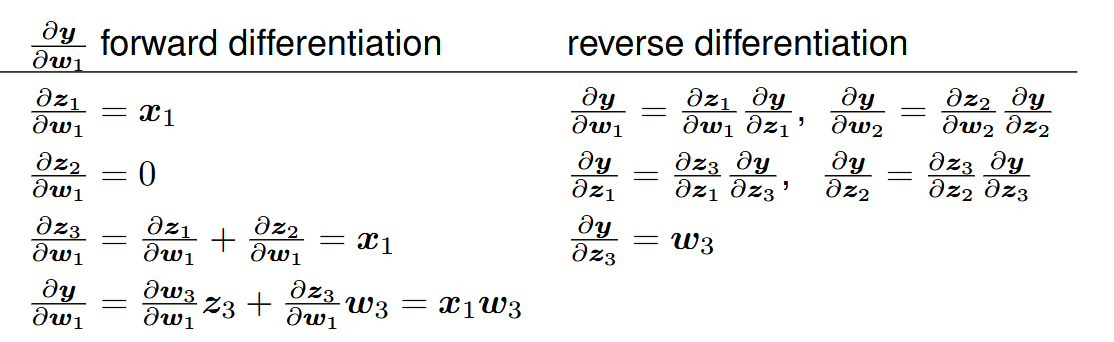
\includegraphics[scale=0.2]{contents/imgs/Screenshot 2024-12-26 151230.png}\\
%For $y=w_3(w_2x_2+w_1x_1)$
\begin{itemize}
    \item Computing full gradient in forward prop is \(\mathcal{O}\)(\#paramaters) One backprop is \(\mathcal{O}\)(\#outputs)
Backprop in practice (assume L=3)
\end{itemize}
In general for a $W^L$, \(\frac{\partial  L}{\partial \mathbf{W^L}} = \frac{\partial L}{\partial \hat{y}} \mathbf{h}^\top\). For a \textbf{generic layer} $z=\mathbf{W}x$: \(\frac{\partial L}{\partial z} x^\top\)\\
Thus:  \(\frac{\partial L}{\partial \mathbf{W_2}}=  \frac{\partial L}{\partial \mathbf{z_2}}h_1^\top\) and \(\frac{\partial L}{\partial \mathbf{W_1}}=  \frac{\partial L}{\partial \mathbf{z_1}}x^\top\) \quad \(\frac{\partial L}{\partial \mathbf{z_1}}=  \frac{\partial L}{\partial \mathbf{h_1}} \odot \overset{.}{\phi} (z_1)\)

\subsection{Gradient Descent  \(\theta^{t+1}=\theta^t-\eta\nabla h(\theta^t)\)}
\textbf{Gradient Flow:}
$\frac{d \theta}{dt}=- \nabla h(\theta)$. Gradient flow is ideal trajectory to follow. 
\textbf{Remark:} Gradient descent is a discrete approximation of gradient flow.\\
GD only successful if gradient change slowly in paramater space. \\
\textbf{Smoothness:}
Function $h$ is called $L$-smooth, if for $L>0$ s.t.:
$\Vert \nabla h(\theta_1) - \nabla h(\theta_2) \Vert \leq L \Vert \theta_1 - \theta_2 \Vert \quad (\forall \, \theta_1, \theta_2).$
In terms of gradient descent: the euc norm of gradient differences cannot grow more than linearly in the euc distance in parameter space this is \(\equiv \lambda_{max}(\nabla^2h)\leq L\) or \(\nabla^2h\preceq LI\) \(\forall \theta\)  \\\(\rightarrow\) Both conditions imply that Hessian is bounded above by \(L\) and that Principal eigenvalues correspond to maximum curvature of h. \\
From the Taylor series expansion for some $\theta$ being on the path from $\theta_1$ to $\theta_2$, we get for gradient descent: \\ 
$h(\theta_2) - h(\theta_1) \leq -\eta ||\nabla h(\theta_1)||^2 + \frac{L\eta^2}{2}||\nabla h(\theta_1)||^2 = -\eta\left( 1- \frac{L\eta}{2}\right) || \nabla h(\theta_1)||^2 $\\
\textrightarrow Strict decrease in $h$ guaranteed for $\eta<\frac{2}{L}$; optimal choice is $\eta = \frac{1}{L}$.
\textrightarrow Smoothness and $\eta = \frac{1}{L}$ sufficient to find $\epsilon$-critical \(\equiv ||\nabla h||\leq \epsilon\) point with $O(\epsilon^{-2})$ steps of GD specifically \(t=\frac{2L}{\epsilon^2}(h(\theta^0)-\text{min }h)\)

\textbf{PL-Condition:} A differentiable function $h$ obeys PL condition with parameter $\mu > 0$, iff $\frac{1}{2} \lVert \nabla h(\theta) \rVert^{2} \geq \mu (h(\theta) - \min h) \ (\forall \theta)$. \\
A small gradient norm at param. $\theta$ implies its near optimality. This allows us to use the suboptim. of the solution to ensure fast(er) convergence. \\
\textbf{Proposition.} Let $h$ be differentiable, $L$-smooth and $\mu$-PL. Then gradient descent w/ step size $\eta=1/L$ converges at geometric rate \\
$h(\theta^{t}) - \min h \leq \left( 1 - \frac{\mu}{L} \right)^{t} (h(\theta^{0}) - \min h)$. \\
In DNNs, PL holds not globally, but around a local minimum. Ensures fast convergence, without sub-optimality claims.
Use noisy GD to avoid slow-down close to saddle points.

\subsection{Acceleration \& Adaptivity}
\textbf{Momentum:} Heavy ball overcomes small gradient norms by increasing effective step size;
$\theta^{t+1} = \theta^t - \eta \nabla h(\theta^t) + \beta (\theta^t - \theta^{t-1}), \quad \beta \in (0, 1).$ \\
If the gradient is constant over many steps, then in the limit \\
$\lim_{t \to \infty} (\theta^t - \theta^{t-1}) = - \eta \sum_{i=0}^{\infty} \beta^i \nabla h = - \left[ \frac{\eta}{1 - \beta} \right] \nabla h.$ Large momentum boosts the effective step size by an arbitrarily large factor.

\textbf{Nesterov:} Evaluates the gradient at the extrapolated point\\
$\nu^{t+1} = \theta^{t} + \beta (\theta^{t} - \theta^{t-1})$, \ \ 
$\theta^{t+1} = \nu^{t+1} - \eta \nabla h (\nu^{t+1})$. \\
Guarantees convergence for convex
and strongly-convex functions; optimal in the convex case and accelerated in the strongly-convex case.\\
\textbf{Adaptivity:} Adjusts learning rates per parameter using gradient history, as in AdaGrad, which gradually reduces step sizes over time.\\
\textbf{ Adam \& RMSprop:} Adam uses an exponentially
 weighted average to estimate the mean and variance of each partial derivative. \\
 $g_{i}^{t} = \beta g_{i}^{t-1} + \left(1-\beta \right) \partial_{i} h(\theta^{t}), \ \beta \in [0; 1], \ g_{i}^{0} := \partial_{i}h(\theta^{0})$ \\
  $\gamma_{i}^{t} = \alpha \gamma_{i}^{t-1} + \left(1-\alpha \right) [\partial_{i} h(\theta^{t})]^2, \ \alpha \in [0; 1], \ \gamma_{i}^{0} := [\partial_{i}h(\theta^{0})]^2$ with iterate sequence:
 $\theta_{i}^{t+1} = \theta_{i}^{t} - \eta_{i}^{t} g_{i}^{t}, \ \eta_{i}^{t} = \frac{\eta}{\sqrt{\gamma_{i}^{t}}+\delta}$ \\
 Adam without the use of momentum ($\beta =0$) is RMSprop. Gradient in Adam is typically stochastic based on minibatches.
\subsection{Stochastic Gradient Descent}
\textbf{ Minibatches:}
Accelerate learning in DNNs using minibatches. For size $r=1$, SGD writes as follows:
$\theta^{t+1} = \theta^{t} - \eta \nabla h(\theta^{t})(x_{i}, y_{i}), \ i_{t} \sim U[1,s]$\\
\textbf{Bias \& Variance:}
Unbiasedness of update direction (i.e. in expectation the update directon equal the full batch gradient) is important in SGD.\\
$\mathbf{V}[\theta](\mathcal{S}) = \frac{1}{s} \sum_{i=1}^{s} \lVert \nabla h[\theta](\mathcal{S}) - \nabla h[\theta] (x_{i}, y_{i}) \rVert ^{2}$\\
Of importance for convergence is variance around a global/local minima, $\nabla h(\theta^{\ast})=0$